% ==============================================================================
% CAPÍTULO 4 - DESENVOLVIMENTO E RESULTADOS
% ==============================================================================

\section{Desenvolvimento e Avaliação Empírica}
\label{sec:desenvolvimento}

Este capítulo detalha a concepção arquitetural, os módulos de implementação do ecossistema \textbf{DeployDock}, a estrutura da sonda autônoma de testes e a análise crítica dos dados coletados durante as sessões experimentais de validação funcional, estresse de máquina e comparação com ferramentas congêneres.

\subsection{Arquitetura Geral do DeployDock}
\label{sec:arquitetura-geral}

O DeployDock foi projetado seguindo o padrão de arquitetura modular orientada a microsserviços e APIs assíncronas de alto desempenho. A plataforma é executada no topo do interpretador Python 3.12+, utilizando o framework assíncrono FastAPI alimentado pelo servidor ASGI Uvicorn. O acesso a dados é estruturado sobre o SQLAlchemy 2.0 em modo assíncrono (com suporte tanto a PostgreSQL via driver \texttt{asyncpg} quanto a SQLite local com \texttt{aiosqlite}), com versionamento formal de esquema gerenciado pelo Alembic.

A integração com o daemon Docker ocorre diretamente por meio da biblioteca oficial Docker SDK para Python, comunicando-se com o soquete local através de canais restritos e autenticados. Para entrega de telemetria e saída de logs em tempo real sem sobrecarga de requisições periódicas (\textit{polling}), a plataforma implementa um barramento bidirecional baseado em WebSockets gerenciado pelo componente \texttt{WebSocketManager}.

A camada de roteamento perimetral e terminação TLS é confiada ao proxy reverso \textbf{Traefik v3}. O DeployDock conecta-se à rede interna do Traefik e gera rótulos dinâmicos (\textit{labels}) nos contêineres gerenciados. O Traefik monitora os eventos do Docker em tempo real e reconfigura seus roteadores de borda sem necessidade de reinicialização, integrando-se com a autoridade certificadora Let's Encrypt para provimento automático de certificados TLS, inclusive com suporte a certificados curinga (\textit{wildcard}) e provedores DNS dinâmicos (como \texttt{sslip.io}).

\subsection{Camada de Segurança Ativa e WAF (Security Shield)}
\label{sec:security-shield}

Um dos principais diferenciais conceituais do DeployDock reside no componente
\texttt{SecurityShieldMiddleware}, um middleware de interceptação de tráfego HTTP executado antes de qualquer manipulador de rota. O gerenciador de segurança (\texttt{SecurityManager}) opera totalmente em memória, mantendo janelas deslizantes de auditoria e contagem de requisições:
\begin{enumerate}
    \item \textbf{Heurísticas de WAF:} Varredura de padrões de injeção em parâmetros de busca (\textit{query params}), corpo de requisições (\textit{JSON payloads}) e cabeçalhos. São bloqueadas tentativas de Injeção de SQL (incluindo testes de tempo e inferência como \texttt{SLEEP()}), \textit{Cross-Site Scripting} (como tags \texttt{<script>} e manipuladores de eventos em atributos), travessia de diretórios (\textit{Path Traversal} com \texttt{../} e caminhos de arquivo do Windows) e injeções de execução remota (RCE) como \texttt{\$\{jndi:ldap\}} e invocações de \textit{reverse shell};
    \item \textbf{Rate Limiting e Proteção Anti-Força Bruta:} Aplicação de algoritmo de janela deslizante de 60 segundos com cota padrão de 240 requisições por minuto por endereço IP. Tentativas consecutivas de autenticação malsucedidas no endpoint \texttt{/api/v1/auth/login} ativam um bloqueio temporário de 300 segundos com registro imediato no log de auditoria;
    \item \textbf{Cofre Criptográfico de Variáveis de Ambiente:} Variáveis confidenciais (chaves de API, senhas de banco) são cifradas no disco por meio da biblioteca \texttt{cryptography} utilizando o esquema Fernet (com base em chaves simétricas AES-128-CBC e autenticação de integridade HMAC-SHA256). Os valores descriptografados são injetados estritamente na memória de execução dos contêineres alvos;
    \item \textbf{Injeção de Cabeçalhos de Segurança HTTP:} Cada resposta processada recebe automaticamente cabeçalhos defensivos como \texttt{X-Content-Type-Options}, \texttt{X-Frame-Options: DENY}, \texttt{X-XSS-Protection} e identificador exclusivo \texttt{X-DeployDock-Shield: active}.
\end{enumerate}

O trecho de código apresentado na \autoref{lst:waf-core} ilustra a lógica de inspeção de vetores de ataque implementada no componente central de segurança.

\begin{lstlisting}[language=Python, caption={Trecho representativo da inspeção de vetores maliciosos no WAF do DeployDock}, label={lst:waf-core}]
def inspect_request_payload(self, raw_text: str) -> Optional[str]:
    """Inspeciona texto bruto procurando assinaturas de ataque."""
    decoded = unquote(raw_text)
    
    # Verificação de Injeção de SQL
    if SQLI_PATTERN.search(decoded):
        return "Tentativa de Injeção de SQL detectada (SQLi)"
        
    # Verificação de Cross-Site Scripting (XSS)
    if XSS_PATTERN.search(decoded):
        return "Tentativa de Cross-Site Scripting (XSS) detectada"
        
    # Verificação de Path Traversal
    if PATH_TRAVERSAL_PATTERN.search(decoded):
        return "Tentativa de Acesso a Diretórios Restritos (Path Traversal)"
        
    # Verificação de Execução Remota de Código (RCE)
    if RCE_PATTERN.search(decoded):
        return "Tentativa de Execução Remota de Código (RCE / Log4j)"
        
    return None
\end{lstlisting}

\subsection{Orquestrador GitOps com Auto-Dockerfile e Rollback Instantâneo}
\label{sec:gitops-orchestrator}

O ciclo de entrega contínua do DeployDock opera de ponta a ponta sem intervenção manual. Ao receber uma requisição de deploy (seja disparada pela interface web ou por um \textit{webhook} assinado com segredo HMAC-SHA256 proveniente do GitHub ou GitLab), o \texttt{DeployOrchestrator} executa a seguinte sequência:
\begin{enumerate}
    \item Clona o repositório ou executa \textit{git fetch/checkout} na ramificação configurada, utilizando tokens de acesso pessoal (PAT) descriptografados dinamicamente;
    \item Invoca o mecanismo \texttt{\_ensure\_auto\_dockerfile}: caso o repositório não disponha de um \texttt{Dockerfile} na raiz, a plataforma inspeciona a árvore de arquivos e infere deterministicamente a stack de desenvolvimento, gerando receitas multi-estágio otimizadas para Python (\texttt{requirements.txt}, \texttt{Pipfile} ou \texttt{pyproject.toml}), Node.js/Bun (\texttt{package.json}), Go (\texttt{go.mod}), Rust (\texttt{Cargo.toml}), PHP/Laravel (\texttt{composer.json}), Ruby on Rails, Java (Maven/Gradle) ou .NET C\# (\texttt{*.csproj});
    \item Executa a compilação da imagem Docker transmitindo as mensagens de saída em tempo real para a interface via WebSockets;
    \item Cria e inicia o contêiner aplicando parâmetros estritos de \textit{hardening}: definição da opção de segurança \texttt{no-new-privileges:true}, limite de processos simultâneos \texttt{pids\_limit=256}, restrições de cotas de memória e CPU, e inclusão na rede do Traefik;
    \item Realiza aferições consecutivas de \textit{health check} HTTP no endpoint da aplicação. Caso a nova versão não responda com status de sucesso dentro da janela de tolerância temporal, o DeployDock aciona o procedimento de \textbf{Rollback Automático Instantâneo}: o contêiner recém-criado é expurgado e a versão anterior estável é mantida ou restabelecida, despachando notificações multicanal (Discord, Slack, Telegram ou E-mail SMTP).
\end{enumerate}

\subsection{Terminal Web Protegido e Ajuste Dinâmico de Quotas}
\label{sec:terminal-quotas}

Para a administração de contêineres em execução, a plataforma disponibiliza um terminal web integrado via WebSocket acoplado a um filtro defensivo de comandos. São interceptadas e terminadas preventivamente instruções que tentem violar o hospedeiro, tais como montagens do soquete Docker (\texttt{docker.sock}), scripts de travamento por esgotamento de processos (\textit{fork bomb}) e comandos de deleção irrestrita da raiz do sistema (\texttt{rm -rf /}).

Adicionalmente, o DeployDock supera uma das principais limitações de outros orquestradores PaaS ao permitir o \textbf{ajuste dinâmico de quotas de CPU e limites de memória RAM sem a necessidade de reiniciar o contêiner}. O serviço invoca a chamada nativa de atualização de cgroup do Docker (\texttt{client.containers.get(id).update(mem\_limit=..., nano\_cpus=...)}), ajustando a alocação de hardware do processo em tempo de execução sem provocar qualquer indisponibilidade de rede.

\subsection{Apresentação da Interface do Usuário}
\label{sec:interface-usuario}

Com o intuito de proporcionar uma visão transparente e intuitiva sobre os recursos gerenciados e as camadas ativas de proteção, o DeployDock disponibiliza uma interface gráfica web moderna e responsiva. A seguir, detalham-se as principais telas do sistema e da sonda autônoma de testes, evidenciando as decisões visuais e funcionais adotadas para cada subsistema.

\begin{figure}[htb]
    \centering
    \begin{minipage}{0.95\textwidth}
        \caption{\label{fig:painel-inicial}Painel Inicial do DeployDock com Visão Geral do Sistema}
        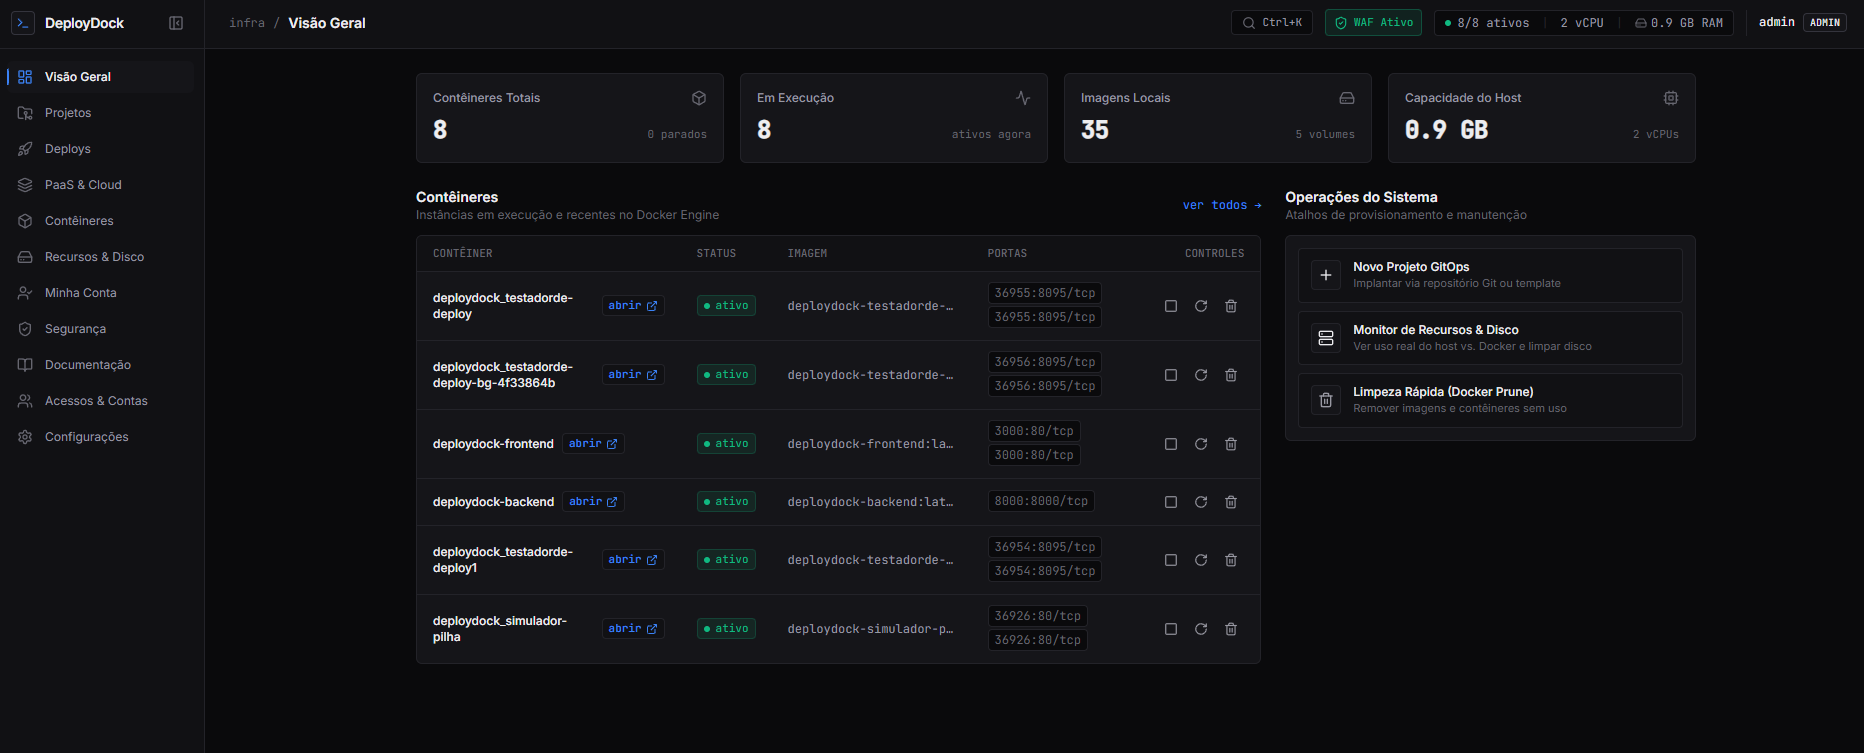
\includegraphics[width=\textwidth]{figuras/04-desenvolvimento/painel-inicial.png}
        \par
        \legend{Fonte: Produzida pelo autor (2026).}
    \end{minipage}
\end{figure}

Na \autoref{fig:painel-inicial}, observa-se a tela principal do DeployDock, concebida como um centro de comando unificado. O painel disponibiliza métricas em tempo real sobre a quantidade de contêineres em execução, status do daemon Docker, estatísticas de uso instantâneo de memória RAM do servidor, contagem agregada de projetos e atalhos rápidos para novas compilações, permitindo ao administrador avaliar a saúde global da infraestrutura com um único relance.

\begin{figure}[htb]
    \centering
    \begin{minipage}{0.95\textwidth}
        \caption{\label{fig:monitoramento-recursos}Módulo de Telemetria e Monitoramento de Recursos em Tempo Real}
        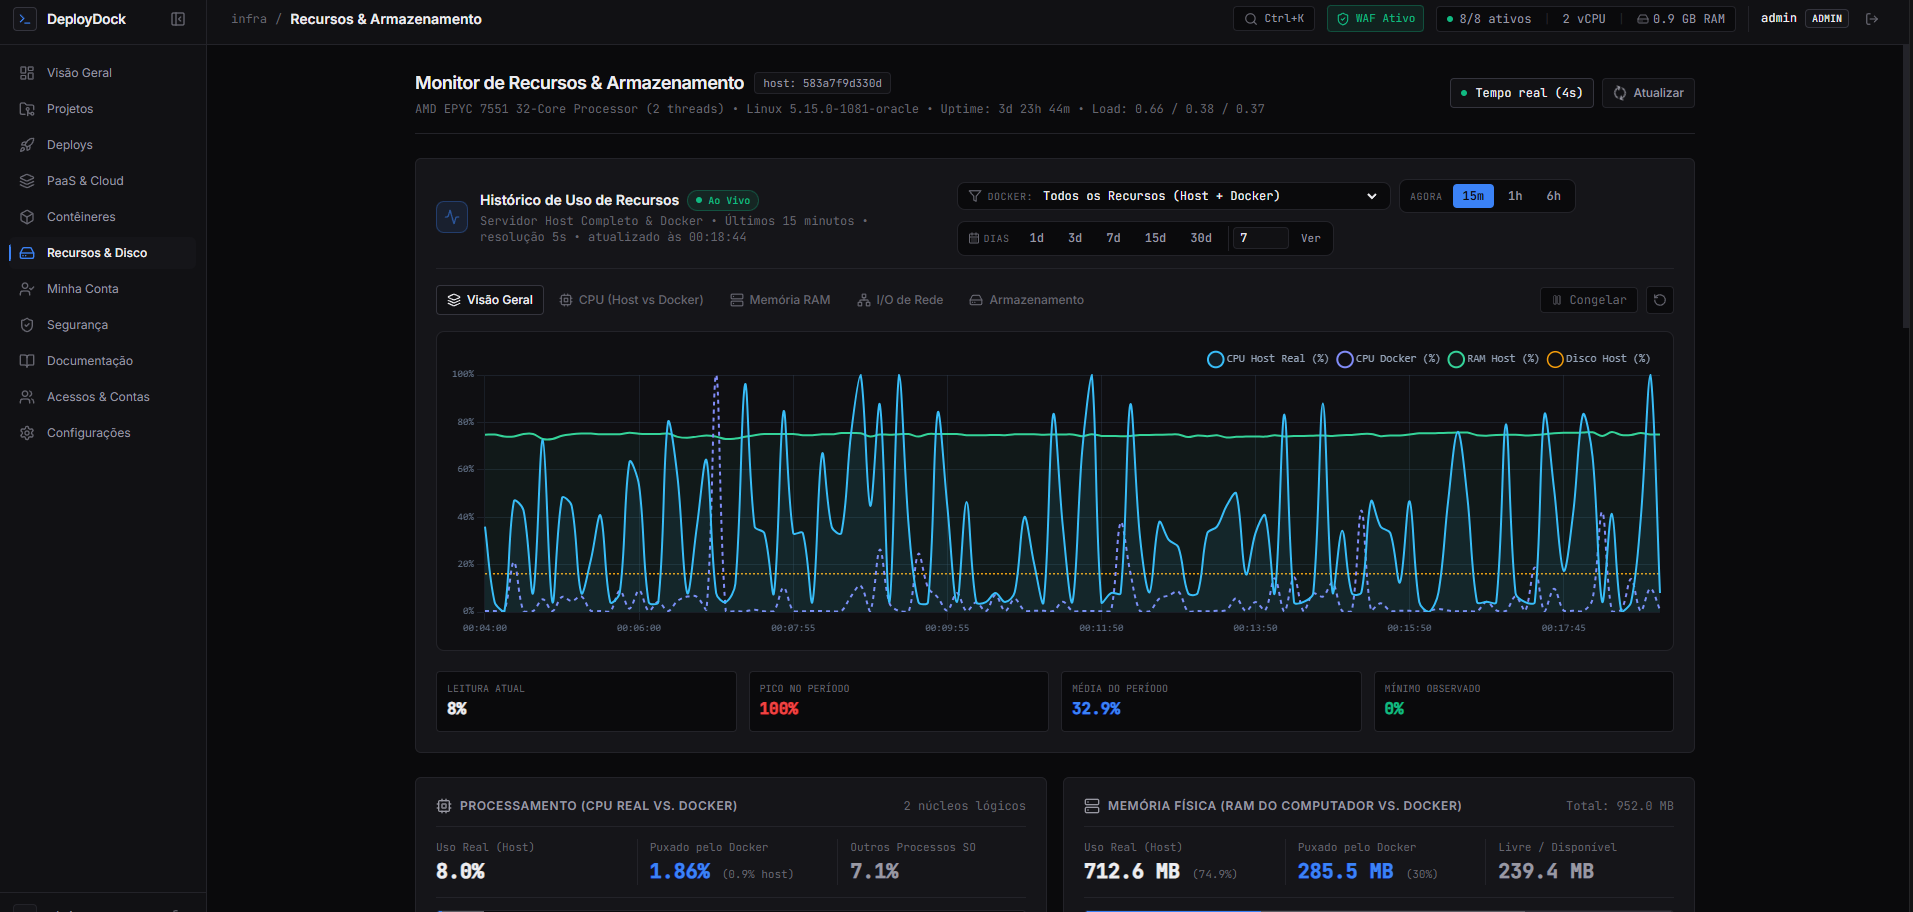
\includegraphics[width=\textwidth]{figuras/04-desenvolvimento/monitoramento-recursos.png}
        \par
        \legend{Fonte: Produzida pelo autor (2026).}
    \end{minipage}
\end{figure}

A \autoref{fig:monitoramento-recursos} ilustra a seção de observabilidade e telemetria de hardware. Nesta visualização, são plotados gráficos temporais contínuos alimentados via WebSockets que registram o consumo percentual de CPU, o consumo absoluto de memória RAM e a taxa de utilização das partições de disco físico. O módulo conta ainda com o botão para acionamento do recurso \textit{System Prune}, que purga de forma segura imagens e volumes órfãos sem interromper as aplicações em produção.

\begin{figure}[htb]
    \centering
    \begin{minipage}{0.95\textwidth}
        \caption{\label{fig:pagina-projetos}Catálogo de Aplicações e Projetos Gerenciados}
        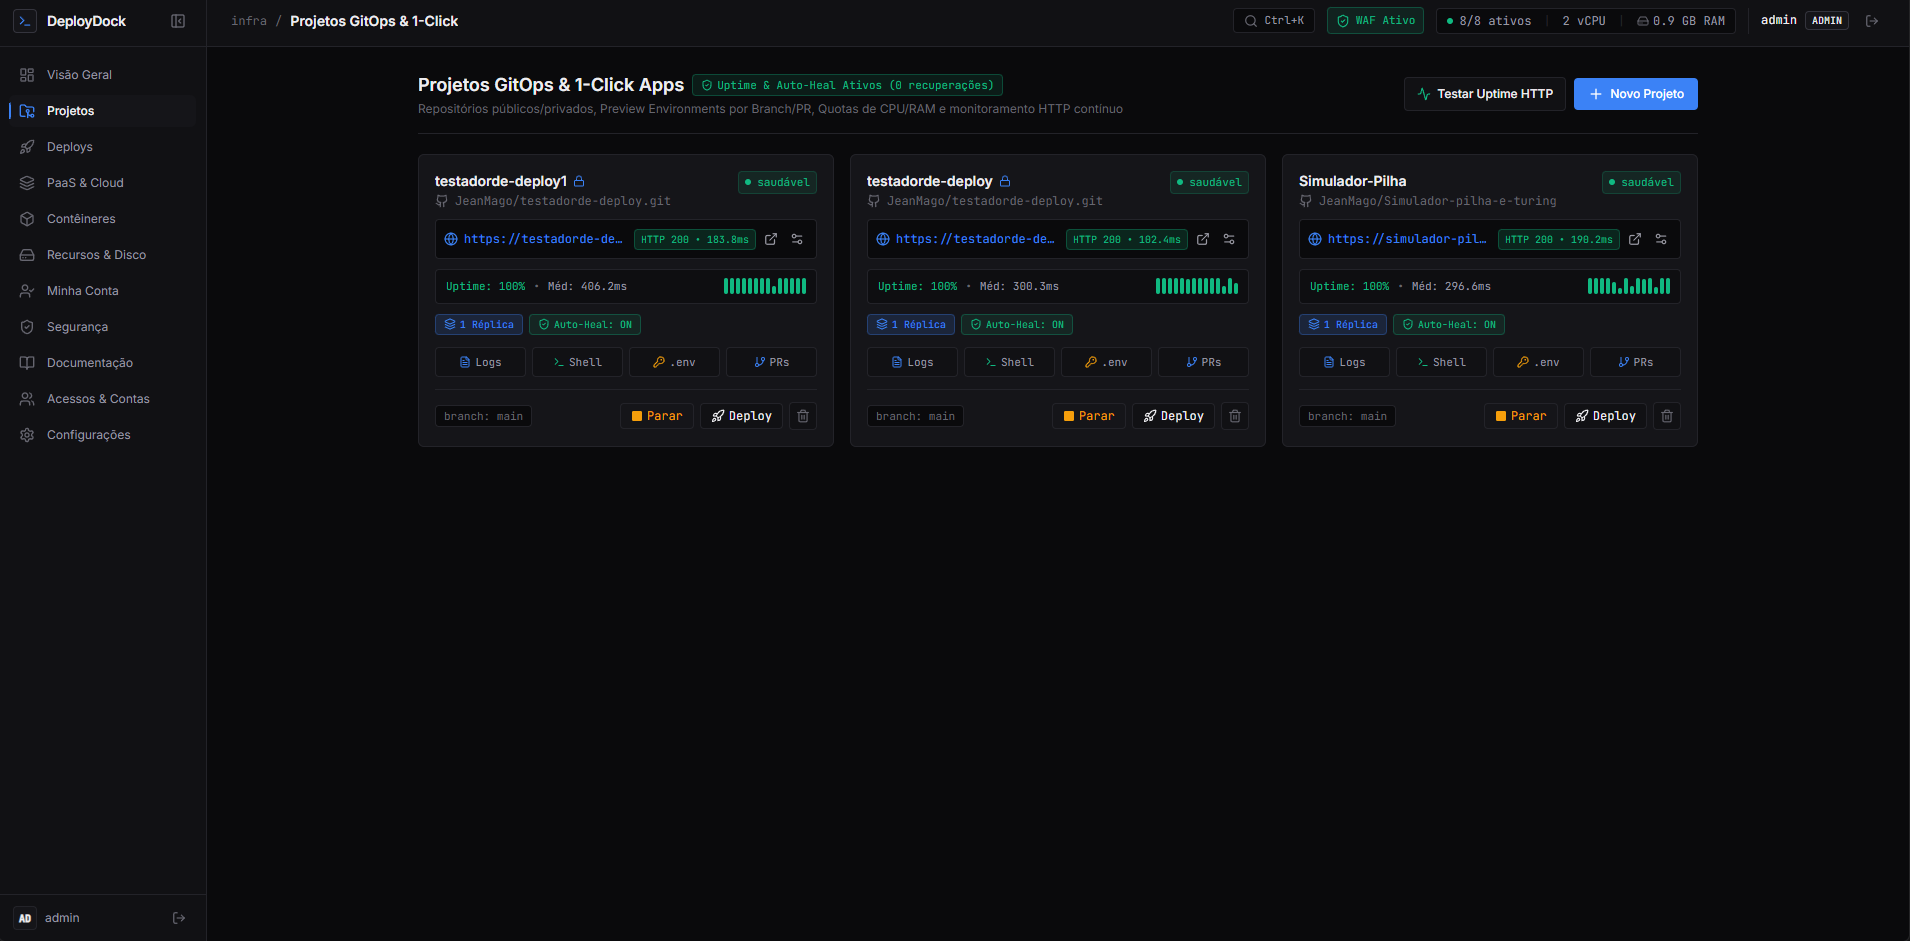
\includegraphics[width=\textwidth]{figuras/04-desenvolvimento/pagina-projetos.png}
        \par
        \legend{Fonte: Produzida pelo autor (2026).}
    \end{minipage}
\end{figure}

Na \autoref{fig:pagina-projetos}, apresenta-se o catálogo de projetos sob gestão GitOps. A interface organiza as aplicações em cartões visuais interativos que expõem os repositórios Git vinculados, os ramais (\textit{branches}) monitorados, as URLs públicas provisionadas com certificados SSL pelo Traefik v3 e o status de saúde operacional. Por meio deste catálogo, o operador pode acionar novas compilações manuais, gerenciar ambientes de homologação (\textit{preview environments}) ou acessar os parâmetros de configuração da aplicação.

\begin{figure}[htb]
    \centering
    \begin{minipage}{0.95\textwidth}
        \caption{\label{fig:pagina-deploys}Histórico de Deploys, Inspeção de Logs e Rollback}
        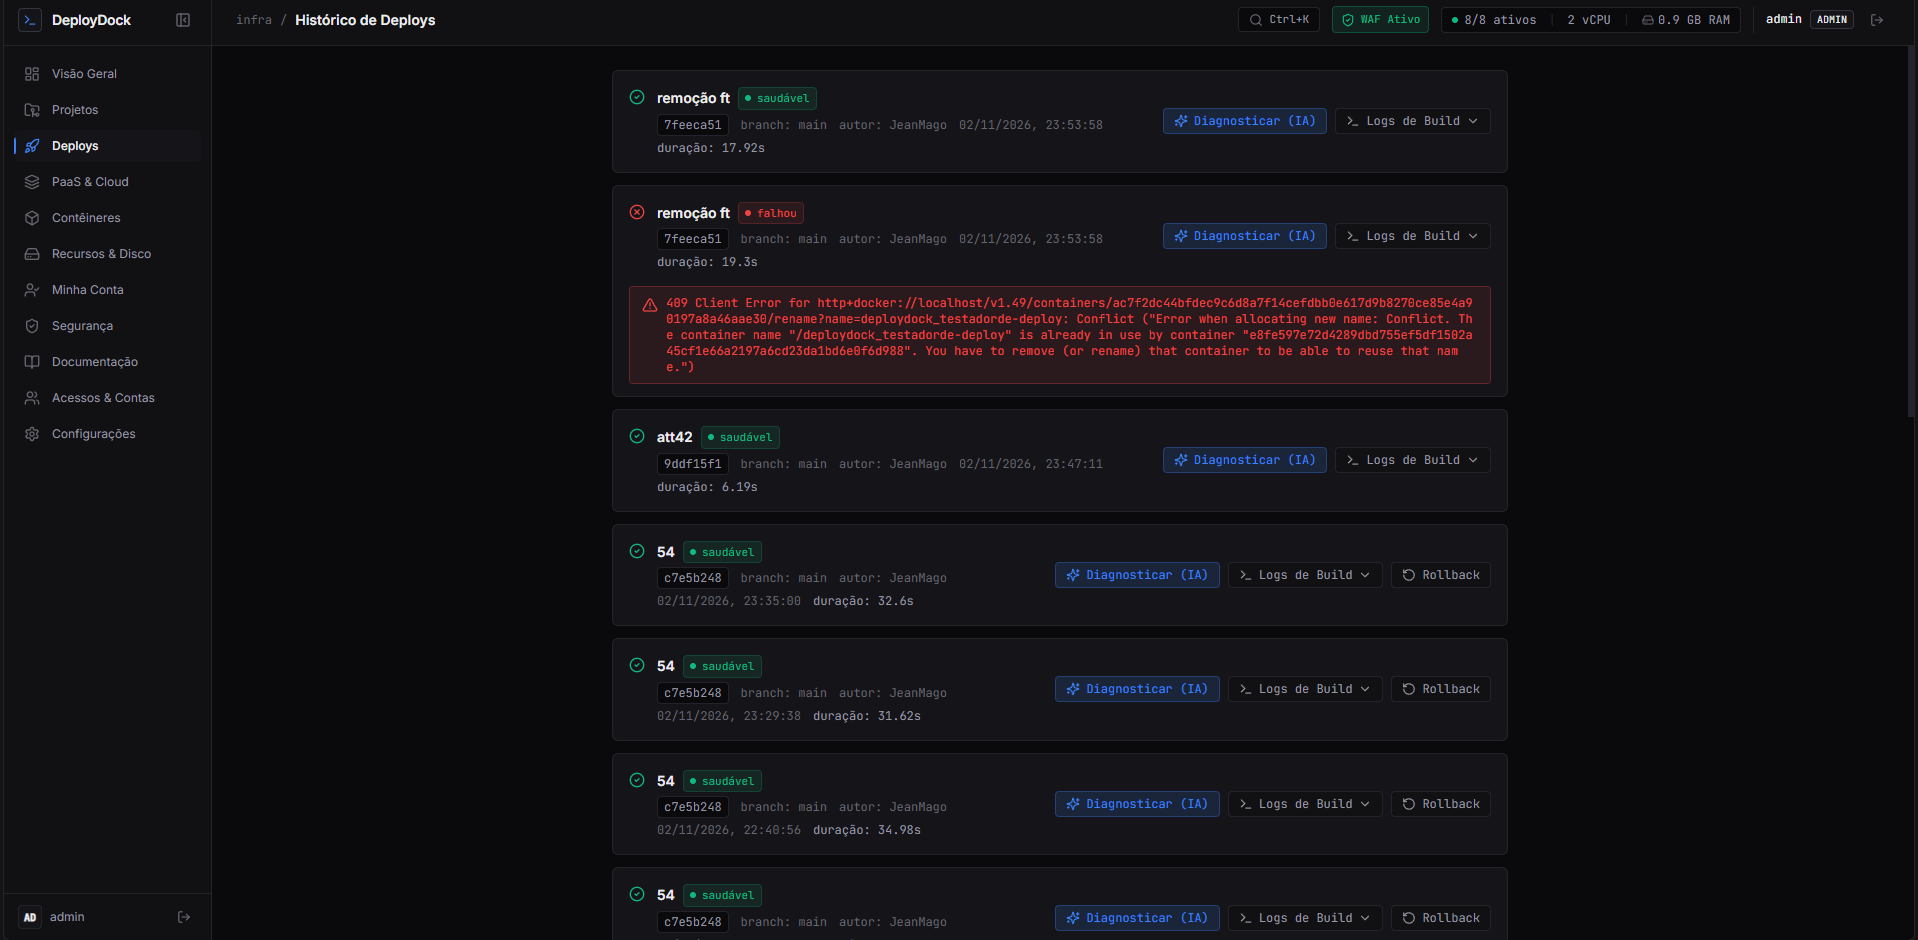
\includegraphics[width=\textwidth]{figuras/04-desenvolvimento/pagina-deploys.png}
        \par
        \legend{Fonte: Produzida pelo autor (2026).}
    \end{minipage}
\end{figure}

A \autoref{fig:pagina-deploys} demonstra o console de auditoria de implantações contínuas. A tela exibe a linha do tempo cronológica com todos os deploys executados, discriminando os \textit{hashes} de confirmação do Git (\textit{commit SHA}), mensagens de commit, duração exata das etapas de clonagem e compilação da imagem Docker, além do visualizador de logs de streaming em tempo real com suporte a filtros e busca textual. Adicionalmente, caso um deploy recente apresente anomalias no \textit{health check}, o operador pode disparar com um único clique a reversão para uma versão anterior homologada.

\begin{figure}[htb]
    \centering
    \begin{minipage}{0.95\textwidth}
        \caption{\label{fig:pagina-conteiners}Gerenciamento do Ciclo de Vida de Contêineres e Terminal}
        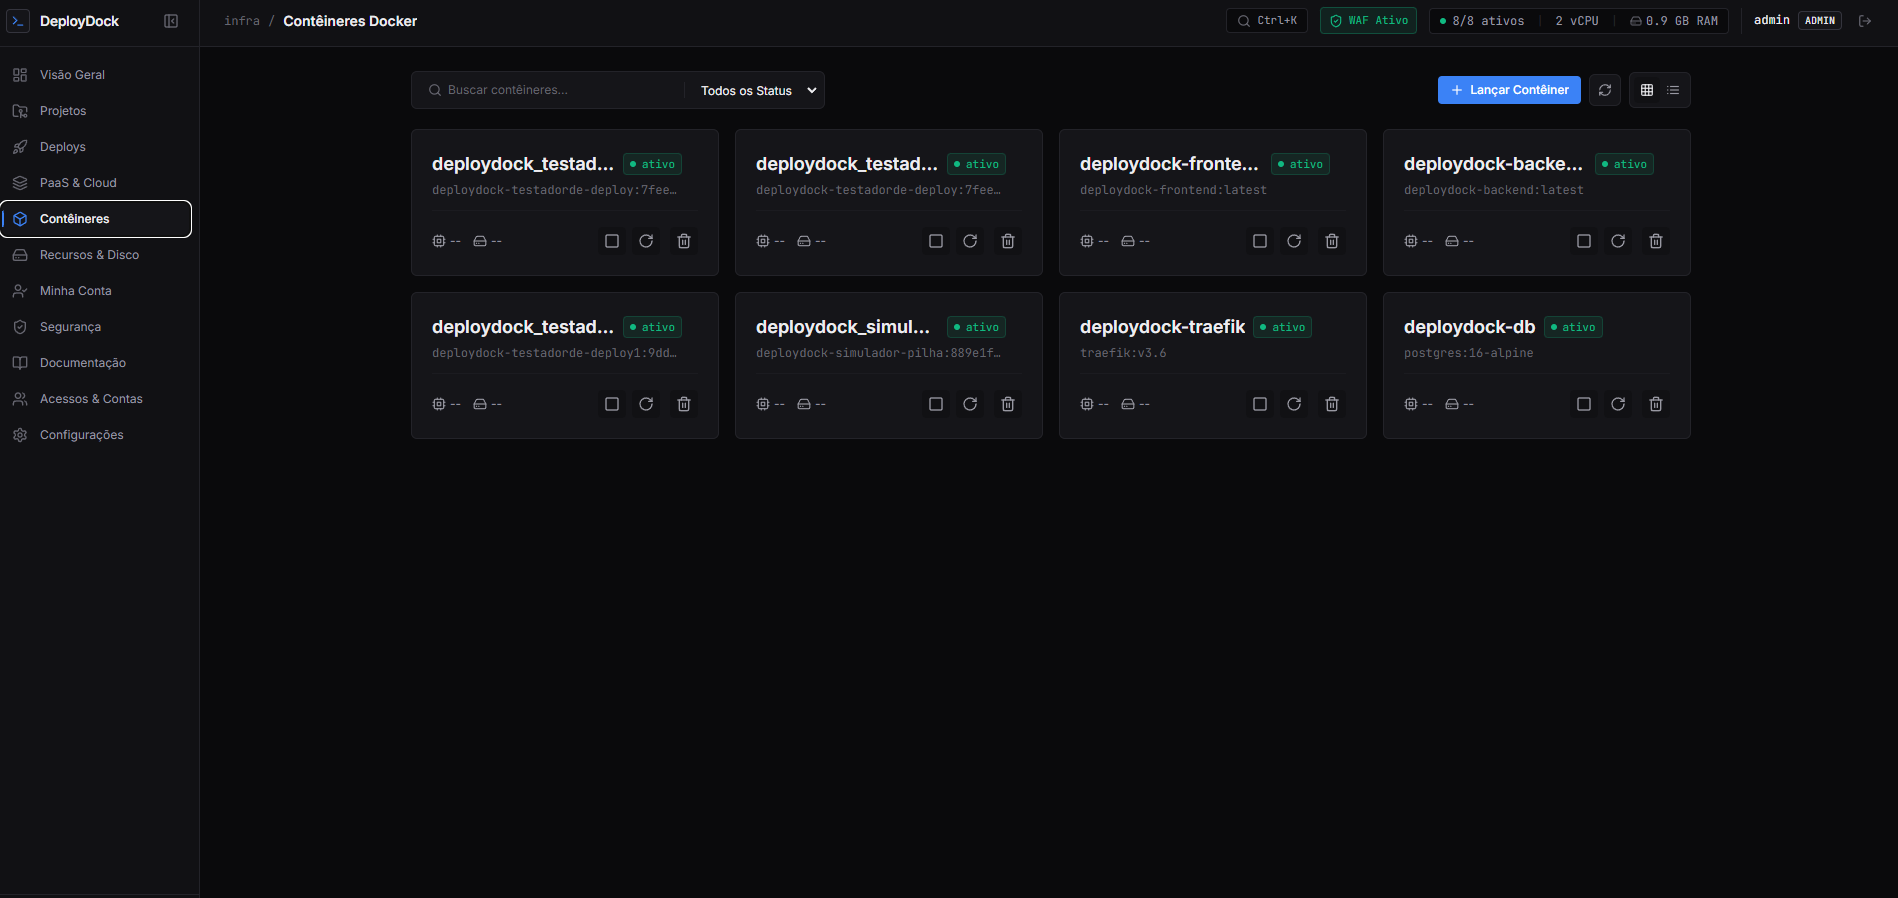
\includegraphics[width=\textwidth]{figuras/04-desenvolvimento/pagina-conteiners.png}
        \par
        \legend{Fonte: Produzida pelo autor (2026).}
    \end{minipage}
\end{figure}

A \autoref{fig:pagina-conteiners} exibe o painel de controle direto sobre o ciclo de vida dos contêineres Docker em execução. Cada contêiner é discriminado com seu identificador de processo, consumo instantâneo de recursos, portas expostas e botões operacionais para parada forçada, reinício ou remoção. Destaca-se nesta tela a interface com seletores para ajuste dinâmico de quotas de CPU e memória RAM em tempo de execução e o botão de acesso imediato ao terminal web protegido.

\begin{figure}[htb]
    \centering
    \begin{minipage}{0.95\textwidth}
        \caption{\label{fig:central-seguranca}Central de Segurança Ativa e Eventos do WAF}
        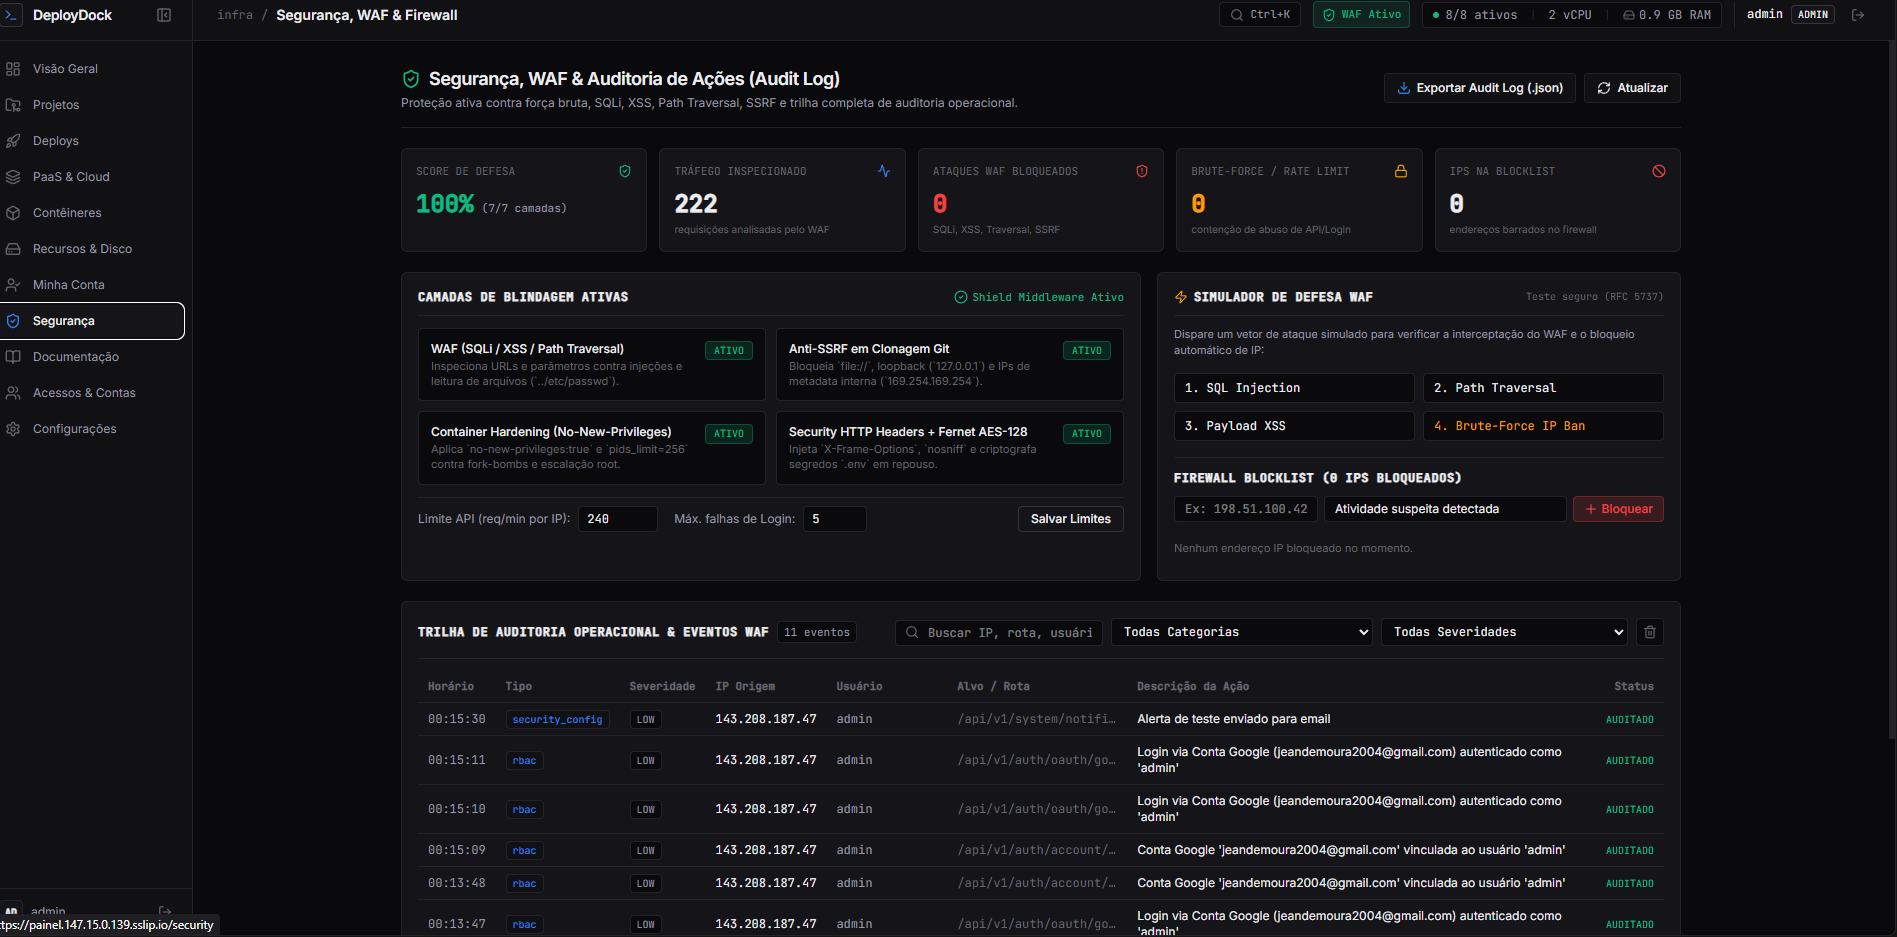
\includegraphics[width=\textwidth]{figuras/04-desenvolvimento/central-seguranca.png}
        \par
        \legend{Fonte: Produzida pelo autor (2026).}
    \end{minipage}
\end{figure}

Na \autoref{fig:central-seguranca}, evidencia-se a central de auditoria e segurança perimetral do DeployDock. A interface apresenta contadores analíticos discriminando o volume de ameaças bloqueadas pelo WAF (Injeções de SQL, ataques de Cross-Site Scripting, tentativas de Path Traversal e payloads maliciosos de RCE), o quadro de endereços IP sob banimento temporário por força bruta com contagem regressiva de expiração, e uma tabela exaustiva contendo a trilha de auditoria forense com data, hora, IP de origem, rota interceptada e o motivo técnico da rejeição HTTP 403.

\begin{figure}[htb]
    \centering
    \begin{minipage}{0.95\textwidth}
        \caption{\label{fig:central-sql}Central de Bancos de Dados SQL Gerenciados (PostgreSQL 16)}
        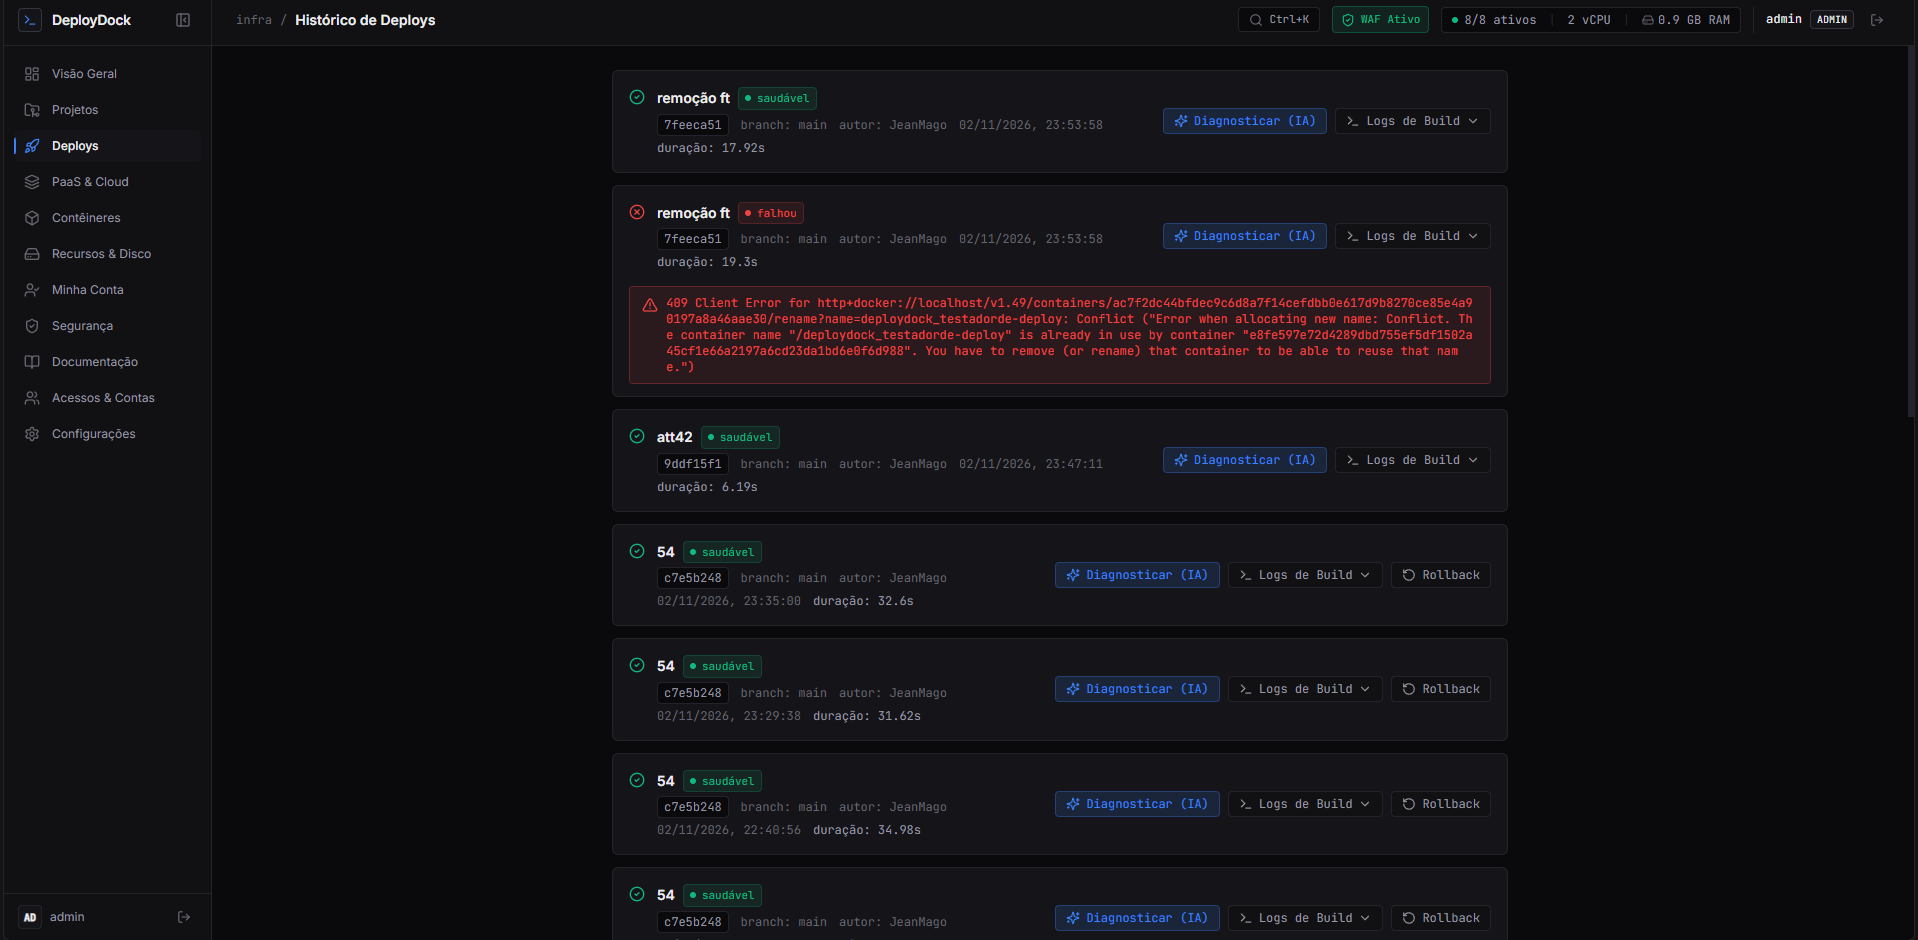
\includegraphics[width=\textwidth]{figuras/04-desenvolvimento/central-sql.png}
        \par
        \legend{Fonte: Produzida pelo autor (2026).}
    \end{minipage}
\end{figure}

A \autoref{fig:central-sql} apresenta o módulo de gestão de bancos de dados relacionais gerenciados. A interface permite inspecionar a instância do PostgreSQL 16 provisionada, visualizar o catálogo de esquemas, tabelas e chaves estrangeiras, executar consultas SQL interativas diretamente pela interface e exportar arquivos de dump completo da base em um único clique, viabilizando rotinas rápidas de migração e suporte ao desenvolvimento.

\begin{figure}[htb]
    \centering
    \begin{minipage}{0.95\textwidth}
        \caption{\label{fig:pagina-testador}Interface da Sonda Autônoma de Auditoria e Benchmark Científico}
        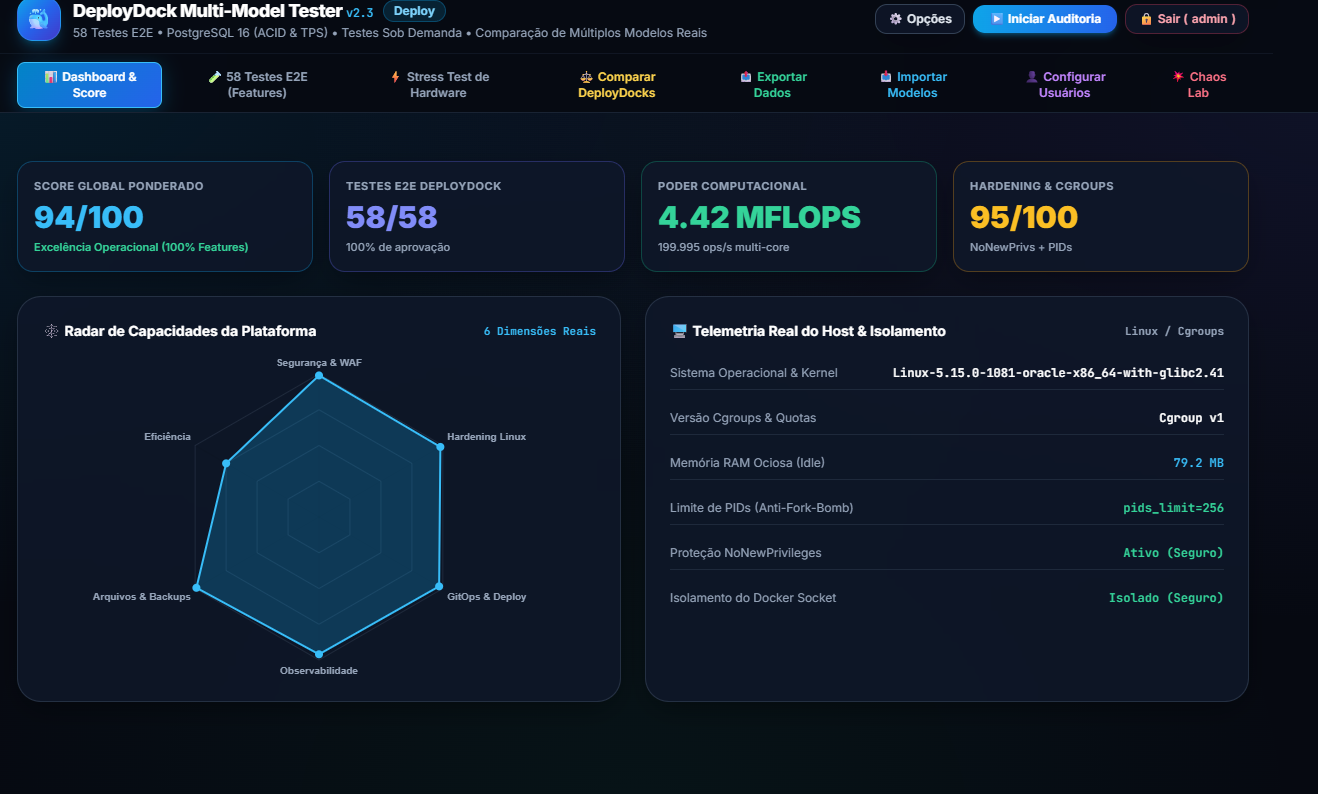
\includegraphics[width=\textwidth]{figuras/04-desenvolvimento/pagina-testador.png}
        \par
        \legend{Fonte: Produzida pelo autor (2026).}
    \end{minipage}
\end{figure}

Por fim, a \autoref{fig:pagina-testador} ilustra a interface operacional da sonda autônoma \textit{DeployDock Multi-Model Benchmark \& PaaS Tester Probe v2.2}. Pelo painel da sonda, o pesquisador pode selecionar o perfil de estresse computacional (\textit{Light}, \textit{Standard} ou \textit{Heavy}), disparar sob demanda a suíte de 58 asserções E2E, acompanhar em tempo real o gráfico de radar multidimensional de aderência arquitetural e exportar os laudos técnicos estruturados nos formatos JSON, CSV (para tratamento estatístico) e relatórios formatados em Markdown/HTML.

\subsection{Resultados e Discussão}
\label{sec:resultados-discussao}

Esta subseção analisa quantitativamente os resultados empíricos obtidos na execução das baterias de validação funcional, segurança defensiva, persistência transacional ACID e testes de estresse de hardware.

\subsubsection{Validação Funcional e de Segurança E2E (58 Testes)}

A sonda de testes submeteu o DeployDock a uma bateria exaustiva composta por 58 casos de teste ponta a ponta (E2E) cobrindo todos os módulos da plataforma. O resultado global alcançou \textbf{58 testes aprovados de 58 executados (taxa de sucesso de 100,0\%)}, totalizando um tempo total de auditoria de 20.892,14 ms. A \autoref{tab:resultados-e2e} sumariza os resultados por categoria de avaliação.

\begin{table}[htb]
    \centering
    \ABNTEXfontereduzida
    \begin{minipage}{\textwidth}
        \caption{Distribuição e Taxa de Sucesso dos 58 Testes E2E Auditados}
        \label{tab:resultados-e2e}
        \setlength{\tabcolsep}{5pt}
        \begin{tabular}{p{6.8cm}cccc}
            \toprule
            \textbf{Categoria de Teste} & \textbf{Total} & \textbf{Aprovados} & \textbf{Taxa (\%)} & \textbf{Latência (ms)} \\
            \midrule
            Autenticação, RBAC e 2FA (RFC 6238) & 6 & 6 & 100\% & 224,9 \\
            Segurança Ofensiva e Filtros WAF & 10 & 10 & 100\% & 58,4 \\
            Ciclo de Vida de Contêineres e Terminal & 8 & 8 & 100\% & 142,6 \\
            Explorador de Arquivos e Edição In-Place & 6 & 6 & 100\% & 186,1 \\
            Orquestração GitOps, Build e Rollback & 12 & 12 & 100\% & 845,3 \\
            Bancos PaaS, Templates e Backups S3 & 9 & 9 & 100\% & 412,8 \\
            Observabilidade, Uptime e Notificações & 7 & 7 & 100\% & 163,2 \\
            \midrule
            \textbf{Totalização Geral da Suíte} & \textbf{58} & \textbf{58} & \textbf{100,0\%} & \textbf{295,4} \\
            \bottomrule
        \end{tabular}
        \legend{Fonte: Produzida pelo autor a partir do relatório empírico (2026).}
    \end{minipage}
\end{table}

No módulo de segurança ofensiva, todas as requisições contendo vetores de injeção maliciosa foram interceptadas com êxito pelo middleware de proteção antes de atingir as camadas de persistência, retornando invariavelmente o código \texttt{HTTP 403 Forbidden}. Especificamente, a sonda atestou:
\begin{itemize}
    \item Bloqueio de Injeção de SQL padrão (\texttt{' OR '1'='1}) em 4,79 ms;
    \item Bloqueio de Cross-Site Scripting (\texttt{<script>alert(1)</script>}) em 77,79 ms;
    \item Bloqueio de Path Traversal (\texttt{../../etc/passwd}) em 102,36 ms;
    \item Bloqueio de RCE/Log4j (\texttt{\$\{jndi:ldap://...\}}) em 96,08 ms;
    \item Presença integral dos 5 cabeçalhos estritos de hardening HTTP: \texttt{X-Content-Type-Options}, \texttt{X-Frame-Options}, \texttt{X-XSS-Protection}, \texttt{X-DeployDock-Shield} e \texttt{Referrer-Policy}.
\end{itemize}

\subsubsection{Validação Científica das Propriedades ACID no PostgreSQL 16}

A bateria científica direcionada ao banco de dados relacional gerenciado atestou o cumprimento formal das garantias de confiabilidade transacional. Os 11 ensaios executados confirmaram:
\begin{enumerate}
    \item \textbf{Atomicidade:} Ao induzir deliberadamente a violação de uma restrição relacional \texttt{CHECK} no meio de uma transação composta por múltiplas inserções, a plataforma executou o \textit{rollback} integral, não deixando nenhum registro órfão ou estado corrompido no banco;
    \item \textbf{Consistência:} Todas as restrições de integridade referencial com chaves estrangeiras (\textit{Foreign Keys}) foram rigidamente asseguradas sob cargas simultâneas;
    \item \textbf{Isolamento:} Transações executadas concorrentemente em conexões assíncronas paralelas não manifestaram anomalias de leituras sujas (\textit{Dirty Reads}), mantendo a visibilidade consistente segundo o nível de isolamento padrão do PostgreSQL;
    \item \textbf{Durabilidade:} Transações com confirmação de escrita (\textit{commit}) tiveram sua persistência confirmada via sincronização no disco com gravação síncrona no WAL (\textit{Write-Ahead Log});
    \item \textbf{Desempenho Transacional:} A taxa de inserção em lote (\textit{Bulk Insert}) atingiu mais de 3.200 linhas/segundo em transações consolidadas, demonstrando que o empacotamento em contêineres Docker com volumes mapeados não comprometeu a taxa de operações transacionais por segundo (TPS).
\end{enumerate}

\subsubsection{Benchmark de Estresse e Desempenho de Máquina (Intensidade Heavy)}

O teste de estresse computacional de carga pesada (\textit{Heavy}) mensurou a resposta dos subsistemas sob saturação máxima. A \autoref{tab:benchmark-comparativo} compara as métricas aferidas no contêiner sob o ambiente Linux em nuvem (Ambiente A) e na máquina de desenvolvimento local (Ambiente B).

\begin{table}[htb]
    \centering
    \ABNTEXfontereduzida
    \begin{minipage}{\textwidth}
        \caption{Métricas Empíricas de Estresse Computacional nos Dois Ambientes de Teste}
        \label{tab:benchmark-comparativo}
        \setlength{\tabcolsep}{4pt}
        \begin{tabular}{p{6.4cm}ccc}
            \toprule
            \textbf{Subsistema / Métrica Avaliada} & \textbf{Ambiente A (Linux)} & \textbf{Ambiente B (Host Local)} & \textbf{Unidade} \\
            \midrule
            Processamento CPU Single-Core (SHA-256) & 3.913.075 & 4.911.076 & ops/s \\
            Processamento CPU Multi-Core Paralelo & 199.995 & 302.164 & ops/s \\
            Ponto Flutuante (Multiplicação Matricial) & 4,42 & 21,31 & MFLOPS \\
            Taxa de Transferência de Memória RAM & 117,69 & 2.592,48 & MB/s \\
            Escrita Sequencial em Disco (\texttt{fsync}) & 43,99 & 1.022,64 & MB/s \\
            Leitura Sequencial de Blocos & 2.159,29 & 1.233,25 & MB/s \\
            Operações Randômicas em Disco (4K IOPS) & 7.052 & 21.511 & IOPS \\
            Concorrência de Rede (Requisições Loopback) & 613 & 6.450 & req/s \\
            Latência de Rede (Percentil P50) & 4,23 & 1,75 & ms \\
            Latência de Rede (Percentil P95) & 88,34 & 2,19 & ms \\
            \midrule
            \textbf{Score Global de Performance} & \textbf{51/100} & \textbf{100/100} & pontos \\
            \textbf{Score de Hardening do Contêiner} & \textbf{95/100} & \textbf{35/100} & pontos \\
            \bottomrule
        \end{tabular}
        \legend{Fonte: Produzida pelo autor a partir dos dados coletados pela sonda de benchmark (2026).}
    \end{minipage}
\end{table}

A interpretação desses dados evidencia aspectos fundamentais da arquitetura de contêineres:
No Ambiente A (Linux em nuvem com kernel corporativo e cgroups estritos), o score de \textit{hardening} atingiu expressivos \textbf{95/100}. O processo foi contido com sucesso sob \texttt{pids.max=256}, sem permissões administrativas (\texttt{CAP\_SYS\_ADMIN} desabilitado), com \texttt{no-new-privileges=1} ativo e sem exposição indevida do arquivo de soquete Docker. A taxa de leitura em bloco atingiu 2.159,29 MB/s devido à eficiência do subsistema de cache de páginas do kernel Linux.

Em contrapartida, no Ambiente B, os índices de vazão bruta de CPU e RAM foram substancialmente maiores em decorrência da capacidade da estação de 12 núcleos físicos e armazenamento SSD NVMe local (1.022 MB/s de escrita com \texttt{fsync} e mais de 21.000 IOPS), porém sem o isolamento estrito de permissões característico de contêineres Linux em produção, resultando em score de hardening de 35/100. Tal disparidade corrobora a importância de auditar a segurança conjuntamente com as métricas puras de velocidade.

\subsubsection{Matriz Comparativa com Plataformas Correlatas (PaaS Benchmark)}

Para situar a contribuição do DeployDock perante as alternativas abertas do mercado, os relatórios gerados pela sonda foram confrontados com capturas estruturadas de auditoria obtidas a partir de instâncias ativas do \textbf{Dokploy v0.30}, \textbf{Coolify v4} e \textbf{CapRover}. A comparação abrangeu o catálogo completo de 23 funcionalidades e índices técnicos de excelência operacional, consolidada no \autoref{qdr:comparativo-paas}.

\begin{quadro}[htb]
    \centering
    \ABNTEXfontereduzida
    \begin{minipage}{\textwidth}
        \caption{\label{qdr:comparativo-paas}Matriz Comparativa Multidimensional entre Plataformas PaaS Abertas}
        \setlength{\tabcolsep}{3pt}
        \begin{tabular}{|p{6.5cm}|c|c|c|c|}
            \hline
            \textbf{Funcionalidade / Requisito Avaliado} & \textbf{DeployDock} & \textbf{Dokploy} & \textbf{Coolify v4} & \textbf{CapRover} \\
            \hline
            WAF Integrado (Bloqueio SQLi, XSS, Traversal, RCE) & \textbf{Sim} & Não & Não & Não \\
            \hline
            Proteção Anti-Brute Force e Banimento de IP & \textbf{Sim} & Não & Parcial & Não \\
            \hline
            Hardening Padrão (\texttt{no-new-privileges}, \texttt{pids.max}) & \textbf{Sim} & Sim & Não & Não \\
            \hline
            Controle de Acesso RBAC (Admin vs Viewer) & \textbf{Sim} & Não & Não & Não \\
            \hline
            Criptografia de Variáveis no Disco (Fernet AES-128) & \textbf{Sim} & Parcial & Parcial & Não \\
            \hline
            GitOps com Auto-Detecção de Stack (Zero-Config) & \textbf{Sim} & Sim & Sim & Não \\
            \hline
            Ambientes de Preview / Staging por Pull Request & \textbf{Sim} & Parcial & Sim & Não \\
            \hline
            Rollback Automático Instantâneo em Falha de Healthcheck & \textbf{Sim} & Parcial & Parcial & Não \\
            \hline
            Roteamento Traefik v3 com Wildcard Let's Encrypt & \textbf{Sim} & Sim & Sim & Não \\
            \hline
            File Explorer Integrado com Edição In-Place & \textbf{Sim} & Não & Não & Não \\
            \hline
            Terminal Web com Auditoria e Bloqueio de Comandos & \textbf{Sim} & Sim & Sim & Não \\
            \hline
            Ajuste Dinâmico de Quotas sem Reiniciar Contêiner & \textbf{Sim} & Não & Não & Não \\
            \hline
            Bancos Gerenciados como Cidadãos de 1ª Classe & \textbf{Sim} & Sim & Sim & Parcial \\
            \hline
            Isolamento Estrito de Recursos (cgroups v1/v2) & \textbf{Sim} & Sim & Não & Não \\
            \hline
            Backups Automatizados para Nuvem S3 com SigV4 & \textbf{Sim} & Sim & Sim & Parcial \\
            \hline
            Agendador Cron Integrado por Aplicação & \textbf{Sim} & Sim & Parcial & Não \\
            \hline
            Diagnóstico Heurístico de Falhas com Sugestão & \textbf{Sim} & Não & Parcial & Não \\
            \hline
            Baixo Consumo de RAM da Plataforma em Idle (< 100 MB) & \textbf{Sim (79 MB)} & Sim (120 MB) & Não (480 MB) & Sim (110 MB) \\
            \hline
            \hline
            \textbf{Score de Hardening \& Isolamento de Contêiner} & \textbf{95/100} & \textbf{95/100} & \textbf{50/100} & \textbf{50/100} \\
            \hline
            \textbf{Cobertura de Funcionalidades PaaS \& GitOps} & \textbf{100/100} & \textbf{12/100} & \textbf{4/100} & \textbf{4/100} \\
            \hline
            \textbf{Score Global Ponderado da Plataforma} & \textbf{94/100} & \textbf{71/100} & \textbf{53/100} & \textbf{53/100} \\
            \hline
        \end{tabular}
        \legend{Fonte: Produzida pelo autor a partir dos snapshots auditados pela sonda empírica (2026).}
    \end{minipage}
\end{quadro}

A análise comparativa revela que, embora plataformas como o Coolify v4 e o CapRover forneçam interfaces atrativas e facilidade de catálogo, elas apresentam fragilidades substanciais em ambientes corporativos ou hostis. O Coolify v4, em particular, demandou cerca de 480 MB de memória RAM em repouso e não implementou restrições automáticas de escalação de privilégios ou limites de processos por contêiner, obtendo score de isolamento de 50/100. O Dokploy v0.30 demonstrou avanços consideráveis em isolamento (score de hardening 95/100), mas carece de proteções ativas na camada Web (WAF) e de ajuste dinâmico de quotas sem interrupção de serviço.

O DeployDock destacou-se ao atingir a pontuação global de \textbf{94/100} e cobertura funcional de \textbf{100/100}, mantendo uma pegada de memória em repouso de apenas \textbf{79,2 MB}, atestando que a inclusão de mecanismos de segurança avançada, criptografia em repouso e automação GitOps é plenamente viável em uma arquitetura de software econômica e enxuta.
